\chapter{SNAPSHOTS}
\section{Administrator Panel[Server Side]}
\subsection{Login Window}
 \begin{figure}[h!]

\centering

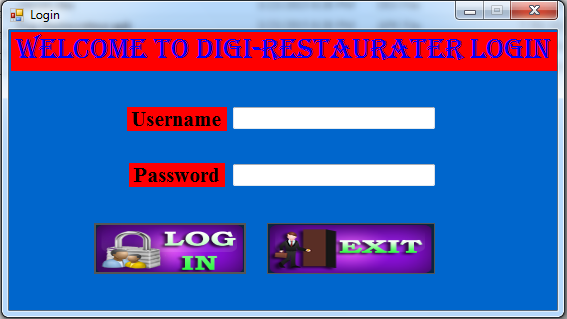
\includegraphics[width=3in]
{1}
\caption{Login Window.}
\end{figure}



\subsection{DashBoard}
Dashboard is nothing but the digi-restaurateur applications home page with this page we can move to any particular forms which are included into the administrator panel which has been controlled by administrator.

 \begin{figure}[h!]

\centering

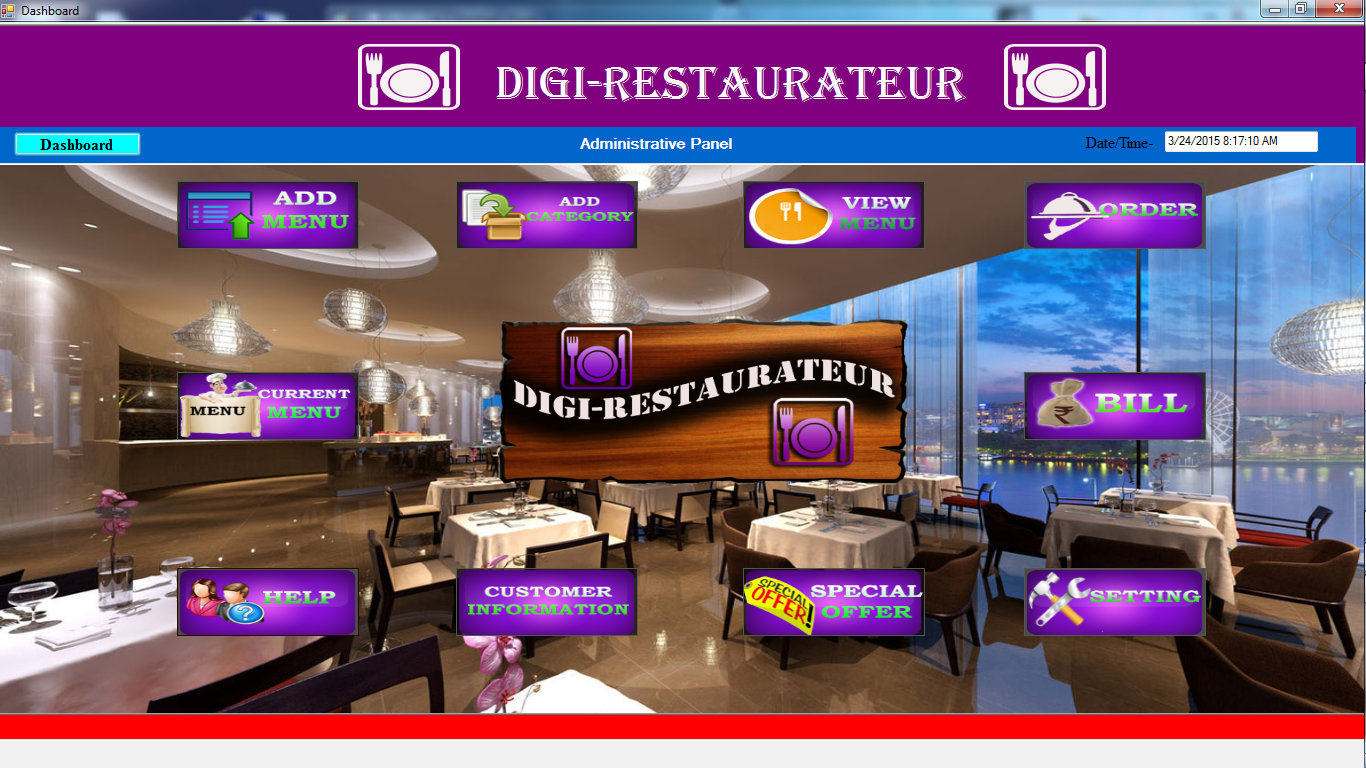
\includegraphics[width=5in]
{2}
\caption{Digi-Restauratuer home panel}
\end{figure}

\subsection{Add Menu Panel}

 \begin{figure}[h!]
\centering
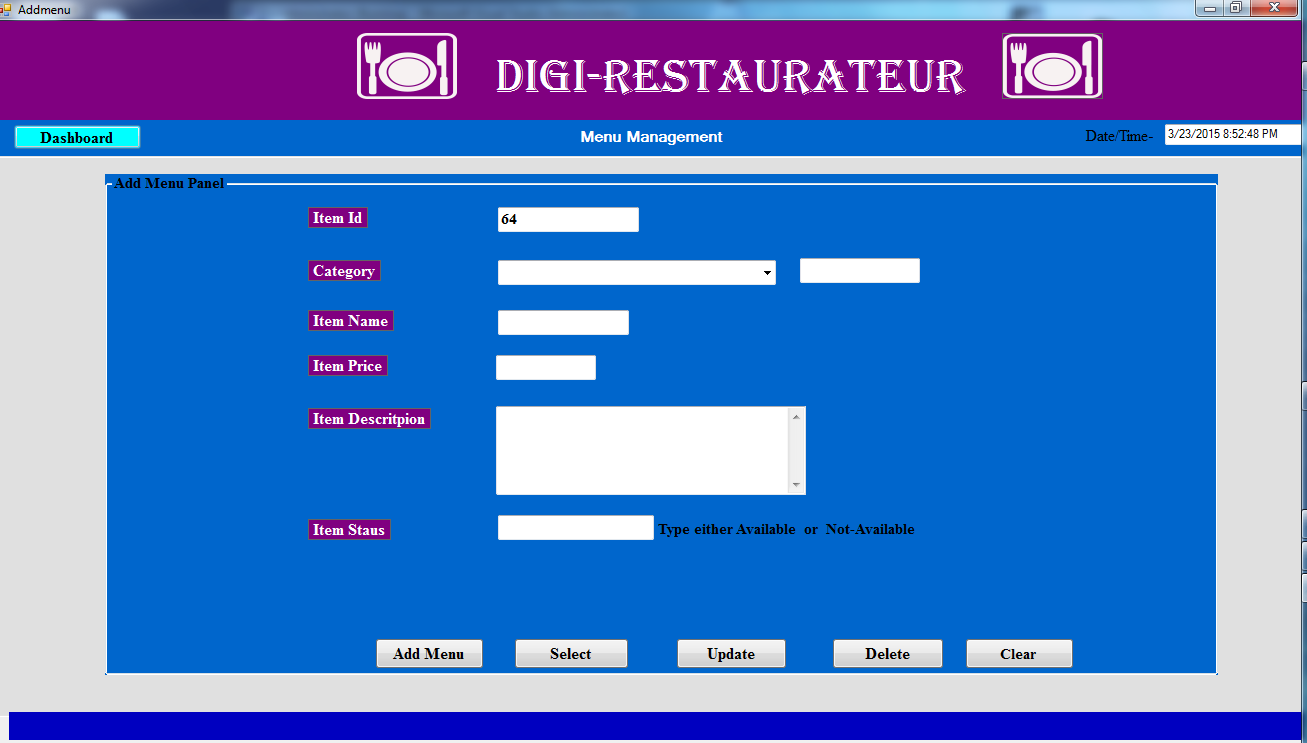
\includegraphics[width=5in]
{3}
\caption{Menu Managmentl}
\end{figure}

\begin{enumerate}
\item {\bfseries Add New Item:}
\begin{itemize}

\item The Itemid will be generated automatically.
 \item Select the category within the combo box.ex.Veg,Non-Veg,Drinks.
 \item Enter the item name.
 \item Enter the item price.
 \item Enter the short description of the item what the actually item will be.
 \item Enter the status of the item as �Available� OR �Not-Available�.
 \item Click on the add menu, it will be added into the database.
\end{itemize}

\item {\bfseries Update Item:}

\begin{itemize}

 \item Enter the item id into the ItemId text field which has been provided in front of item id.
 \item Click on select button it will retrieves the details of your required item.
 \item Then we can modify the records and click on update button it will be saved into the database.
\end{itemize}

\item{\bfseries Delete Item:}

\begin{itemize}
\item Enter the item id into ItemId the text field which has been provided in front of item id.
 \item Click on delete button it will delete the particular record or item.
\end{itemize}

\item{\bfseries Clear Button:}
\begin{itemize}

\item This will be used as clears the text fields to add new items. 
\end{itemize}

\end{enumerate}


\subsection{Add Category Panel}
\begin{figure}[h!]
\centering
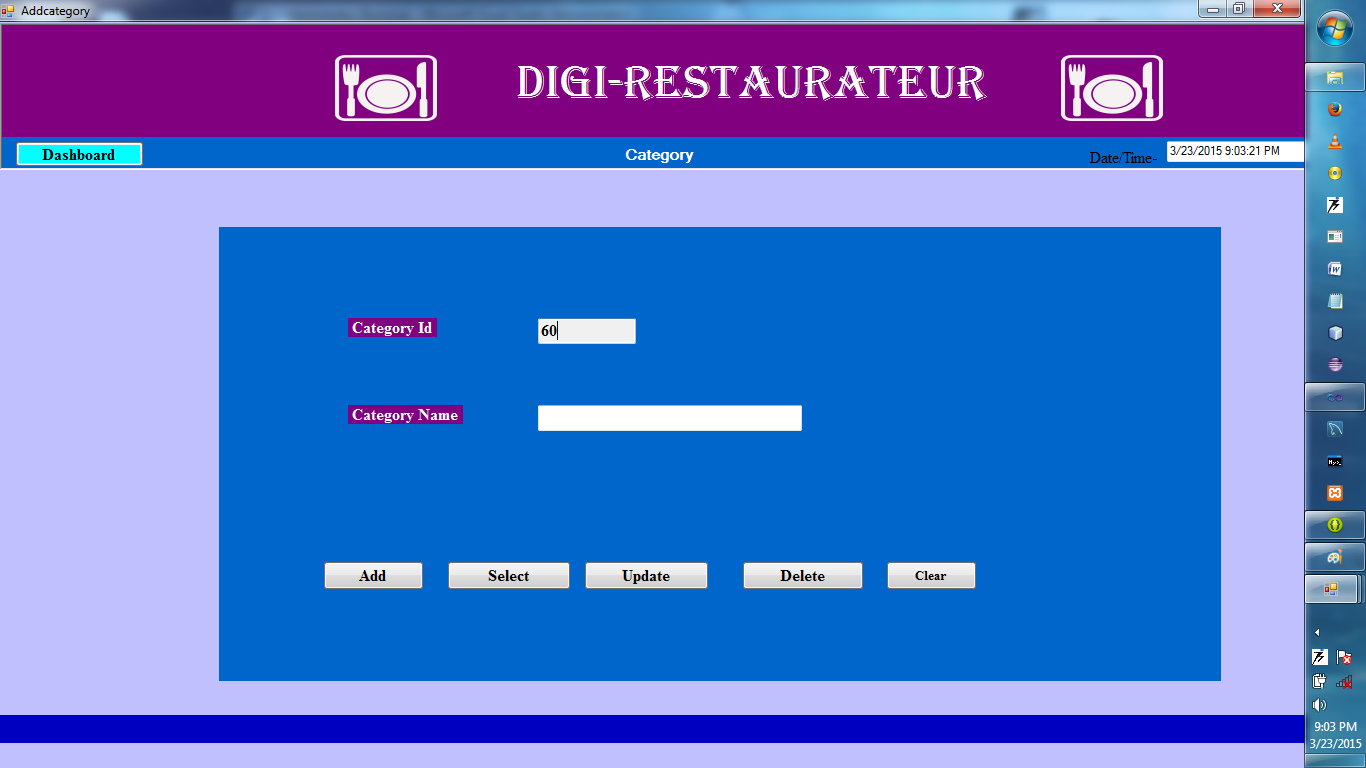
\includegraphics[width=5in]
{4}
\caption{Menu Managmentl}
\end{figure}


{\bfseries Add Category: You can add new category:}
\begin{enumerate}
\item {\bfseries Add New Category:}
\begin{itemize}
 \item The category id will be generated automatically.
 \item Enter the category Name, ex.Veg, Non-Veg.
 \item Click on add button, it will save  into the database as well as this category will added into combo box when new item will be added.
\end{itemize}

\item{\bfseries Select/Update Category:}
\begin{itemize}
\item Enter the category id into the text field which has been provided in front of category id.
 \item Click on select button it will retrieves the details.
 \item Then we can modify the records and click on update button it will be saved into the database.
\end{itemize}

\item{\bfseries Clear Button:}
\begin{itemize}
\item This will be used as clears the text fields to add new category. 
\end{itemize}
\end{enumerate}

\subsection{Currunt Menu Panel}

{\bfseries Current Menus:}
\begin{itemize}
\item View menu panel is one of the important panel of the system which fetch all the records from the database according to category selection.
 \item When we have to fetch a particular category menus, Select category from the combo box it is placed on top of the panel in Middle.
 \item If we select the category  it shows all the items included in that category .
 \item In the data grid view has the check box by default the status has available if you check the box then status will be changed.
 \item The Not-Available status menu can not seen by the customer on a tablet.
\end{itemize}
\begin{figure}[h!]
\centering
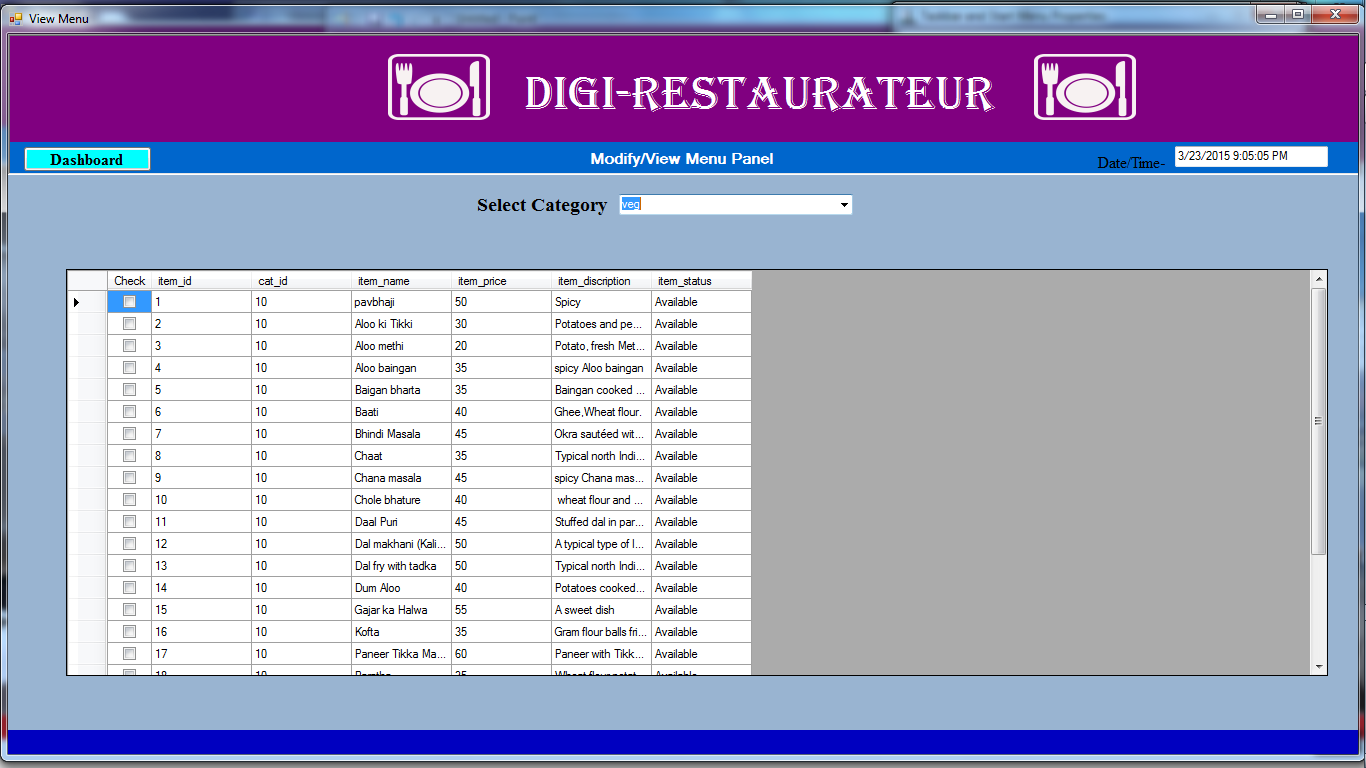
\includegraphics[width=5in]
{5}
\caption{View or Current menus}
\end{figure}

\subsection{Current Orders:}
{\bfseries Current Orders from Customer:}
\begin{itemize}

\item In current order panel it show which orders are coming through the customers they are seen by kitchen or chef.
\item If the chef has checked the checkbox of data grid view for particular item then it will be treated as that menu is complete and status is changed from �Pending� to Billing.

\end {itemize}
\begin{figure}[h!]
\centering
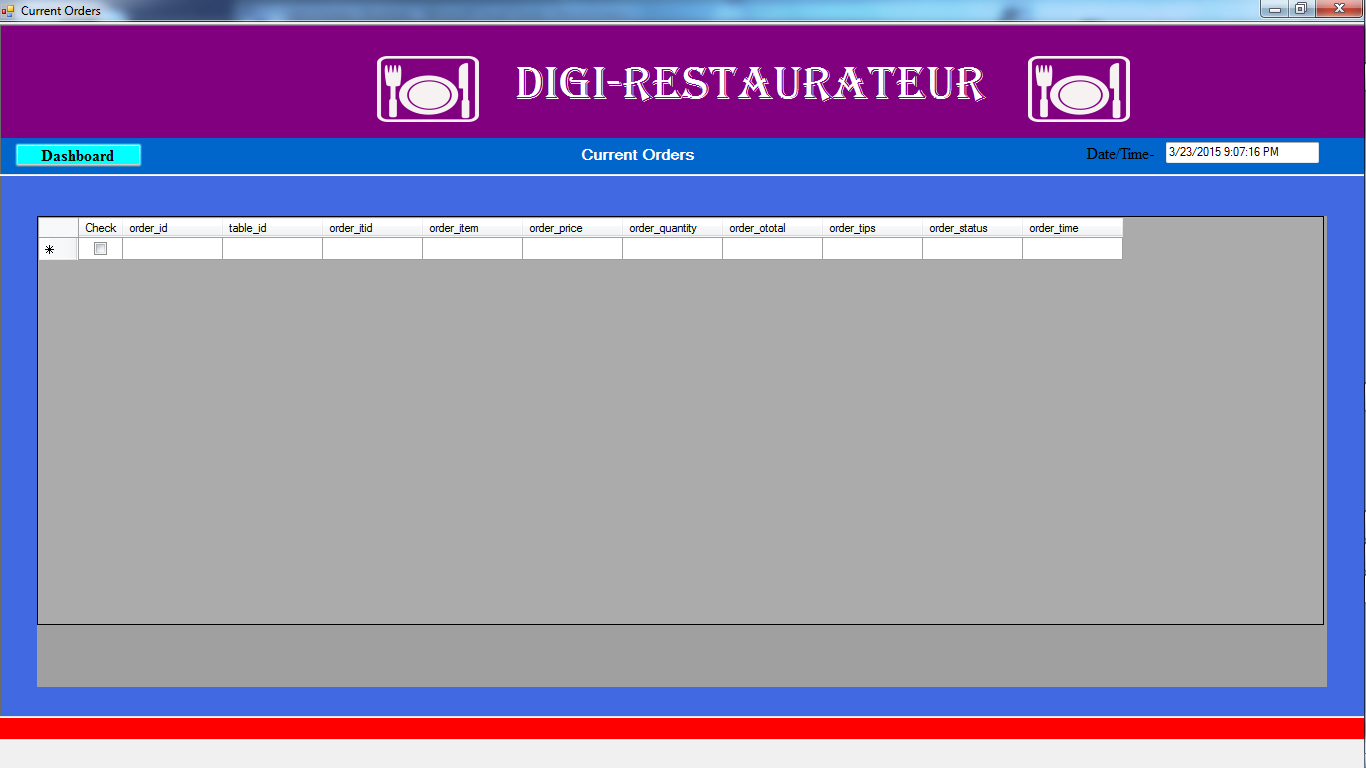
\includegraphics[width=5in]
{6}
\caption{Current Orders}
\end{figure}


\subsection{Current Available Menus:}
{\bfseries Current Menus On The Tablets}
\begin{figure}[h!]
\centering
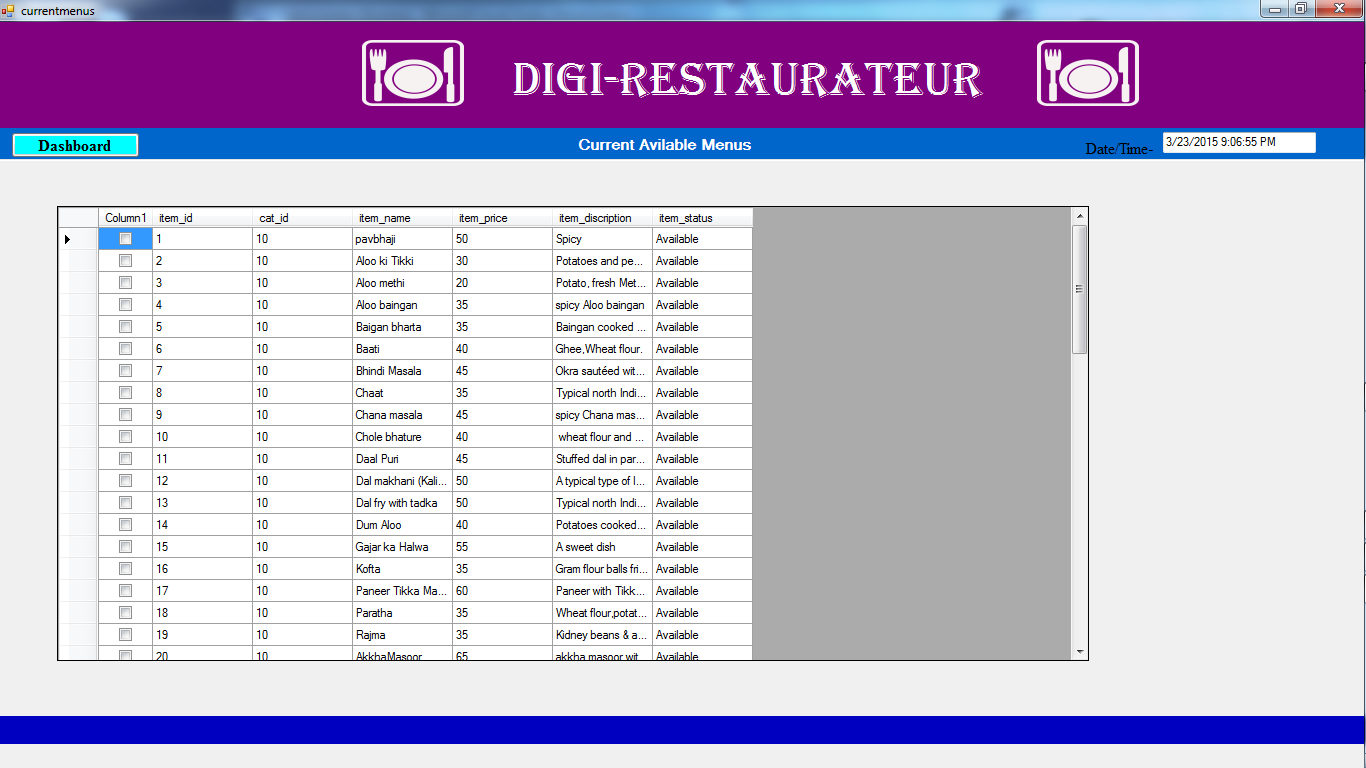
\includegraphics[width=5in]
{7}
\caption{ Current Menus In The List}
\end{figure}

\subsection{Billing Panel}
{\bfseries Customers final bill:}
\begin{figure}[h!]
\centering
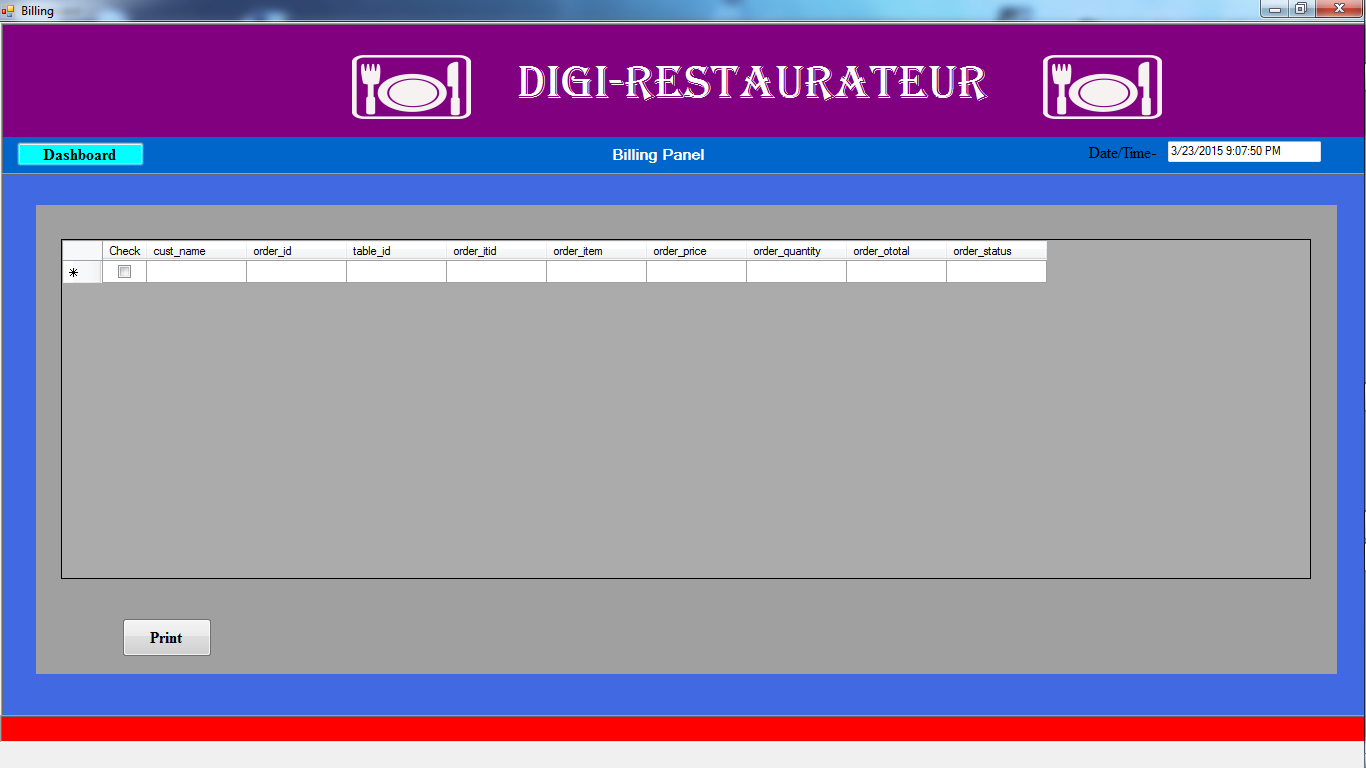
\includegraphics[width=5in]
{8}
\caption{Current Completed Orders.}
\end{figure}
\begin{itemize}
\item The orders which are currently completed state these orders will updates into the billing panel.
\item These orders will sends back to prints the final bill.
\end {itemize}

\subsection{Customer Information}

\begin{itemize}
 \item It contains all the customers� data like customer name, contact number, visit count,feedback.
 \item In customer information the customer visit count also recorded which is used to give discount.
\end{itemize}

\begin{figure}[h!]
\centering
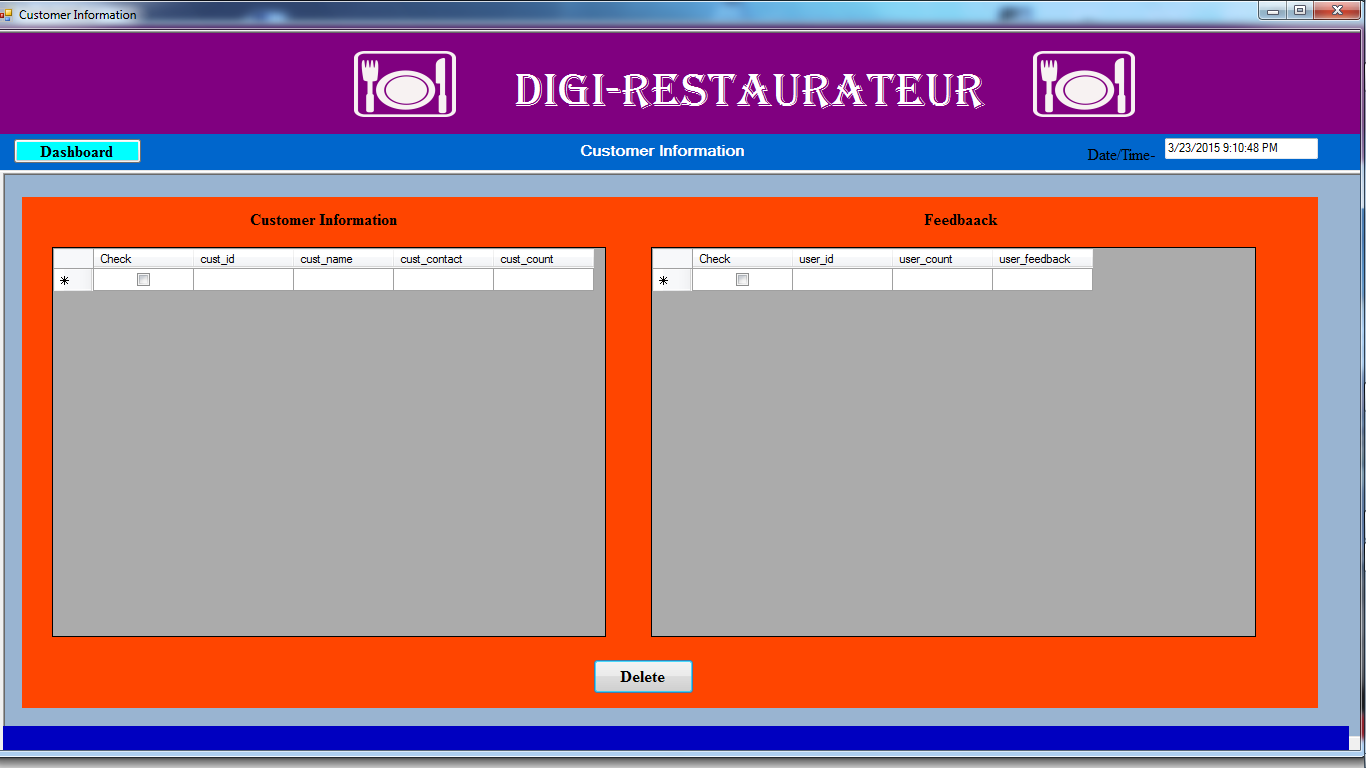
\includegraphics[width=5in]
{10}
\caption{It shows the customer information and feedback.}
\end{figure}

\subsection{Help}
It helps to administrator to use an application
\begin{figure}[h!]
\centering
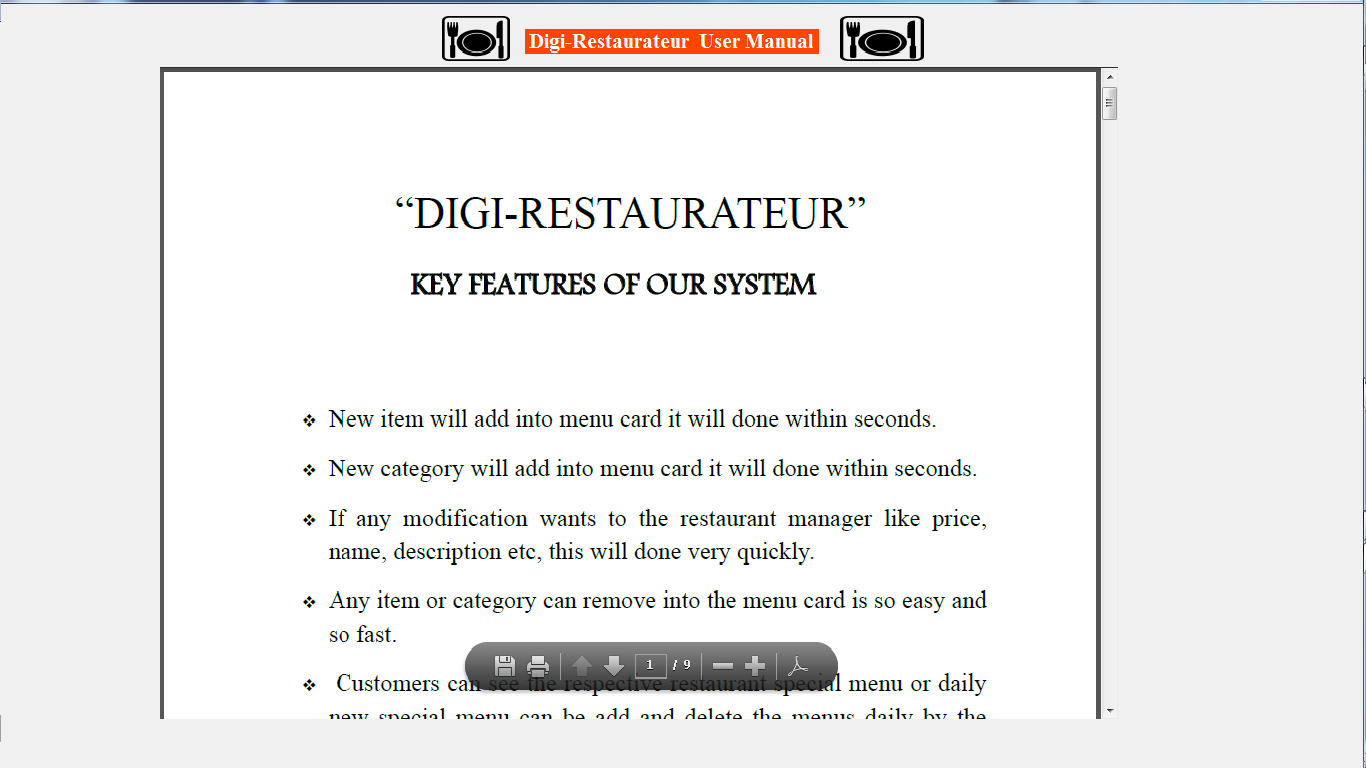
\includegraphics[width=5in]
{9}
\caption{User manual for server side application}
\end{figure}


\subsection{Todays Special Menu}
\begin{itemize}
\item With this panel we can give a daily offers to the customers.
\item also we can provide any new dish which has famous in the restaurant.
\end{itemize}
\begin{figure}[h!]
\centering
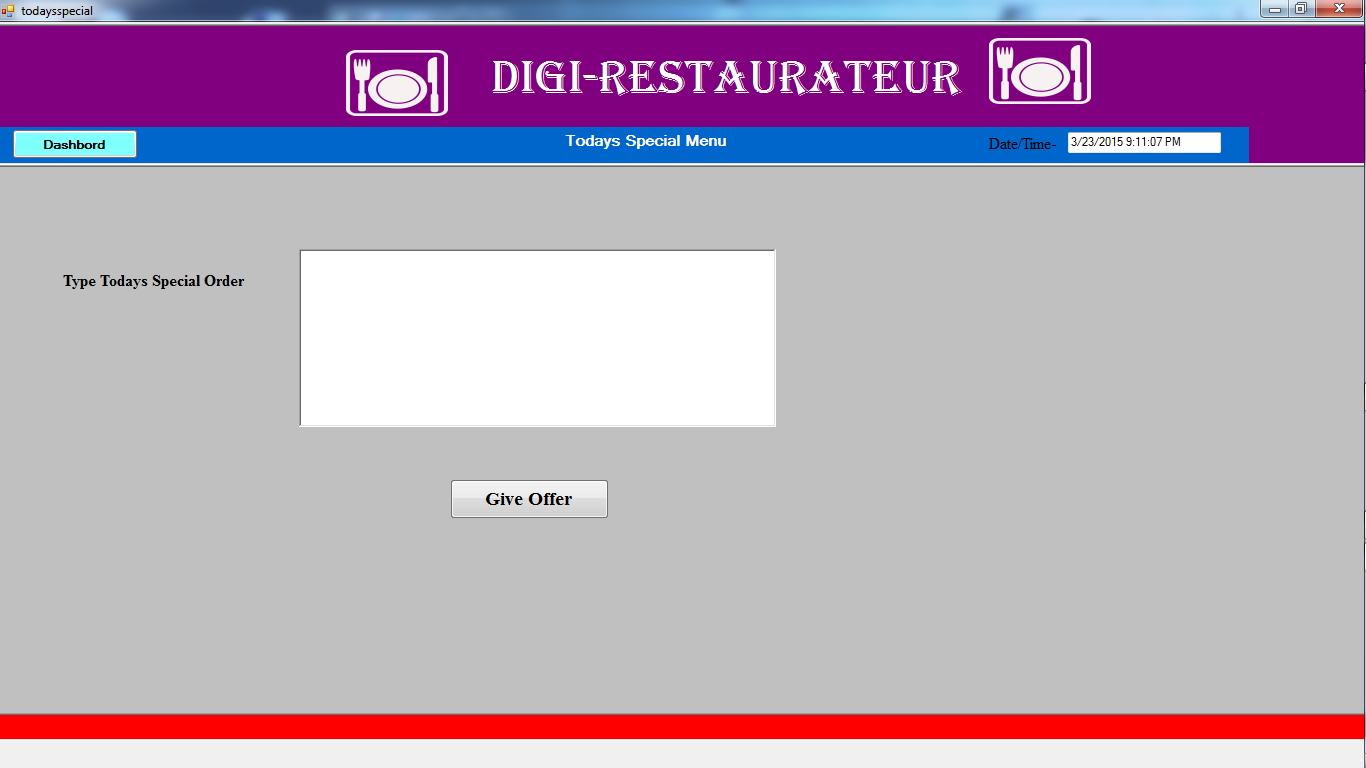
\includegraphics[width=5in]
{11}
\caption{Give the offers to the customers}
\end{figure}


\subsection {Tablet Management:}
\begin{itemize}

\item It will open the tablet, table and waiter management form.
\item Enter the Table Id, Tablet  MAC ADDRESS, Waiter Id  and clicks on the add button, It will added these records in system.
\item If administrator want to delete any tablet or table id�s in the system then he/she can delete the particular data in system.Enter table id in Table Id text box press delete button.
\item If administrator want to update any information then type Table Id in text box click on search button then make changes and press the Update button.
\end{itemize}

\begin{figure}[h!]
\centering
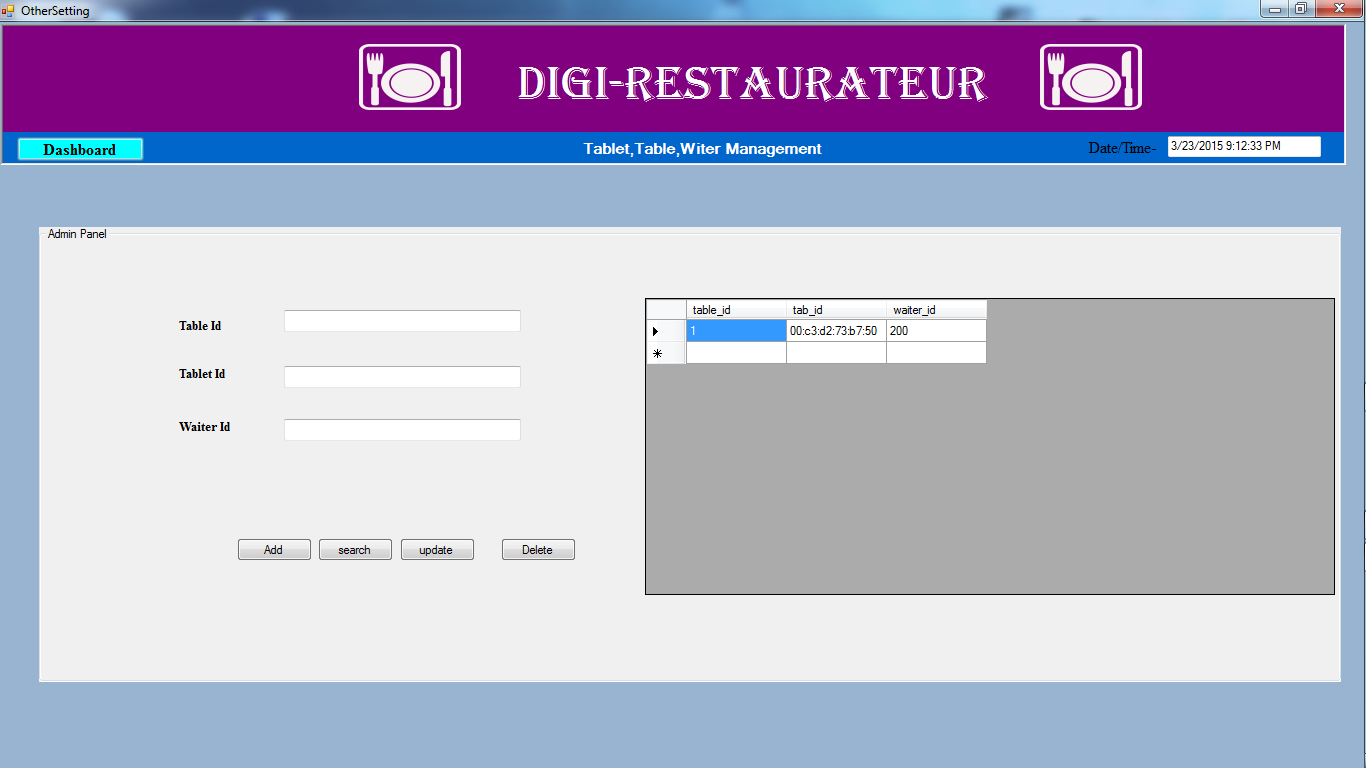
\includegraphics[width=4in]
{14}
\caption{Tablet Management}
\end{figure}


\subsection{Settings: }

\begin{figure}[h!]
\centering
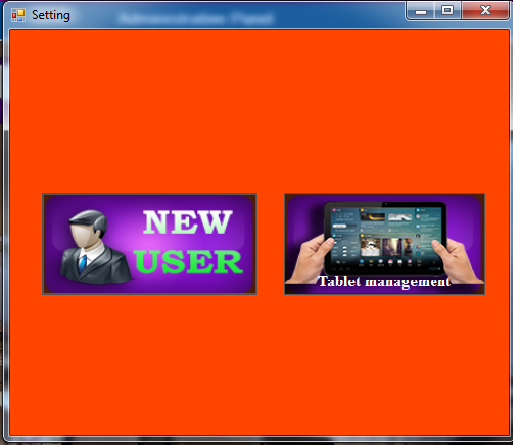
\includegraphics[width=4in]
{12}
\caption{Setting panel}
\end{figure}

\section{Customer Panel [Client Side]}

\begin{figure}[h!]
\centering
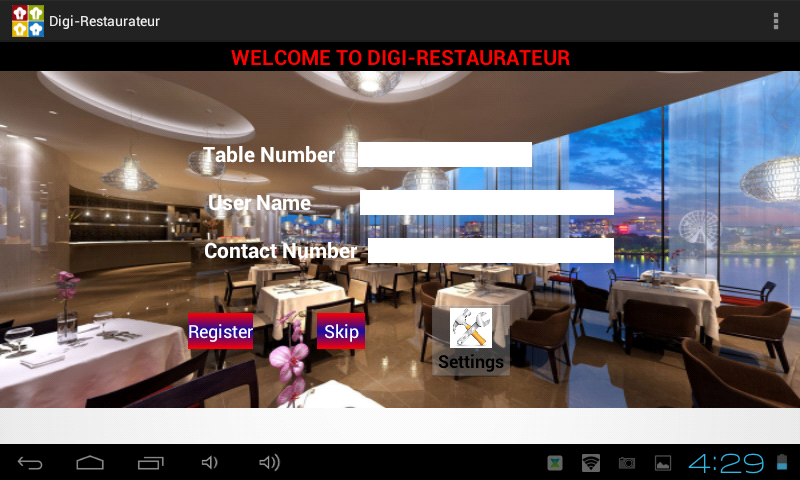
\includegraphics[width=5in]
{t1}
\caption{Registration Window}
\end{figure}


\begin{figure}[h!]
\centering
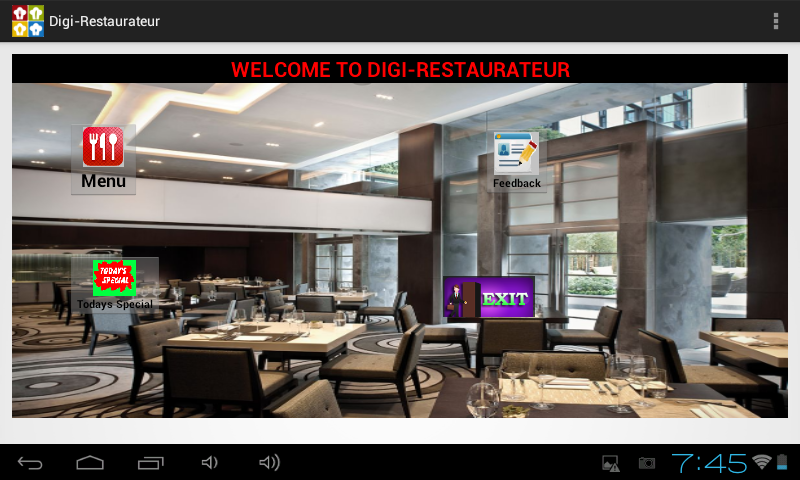
\includegraphics[width=5in]
{t2}
\caption{Home panel}
\end{figure}


\begin{figure}[h!]
\centering
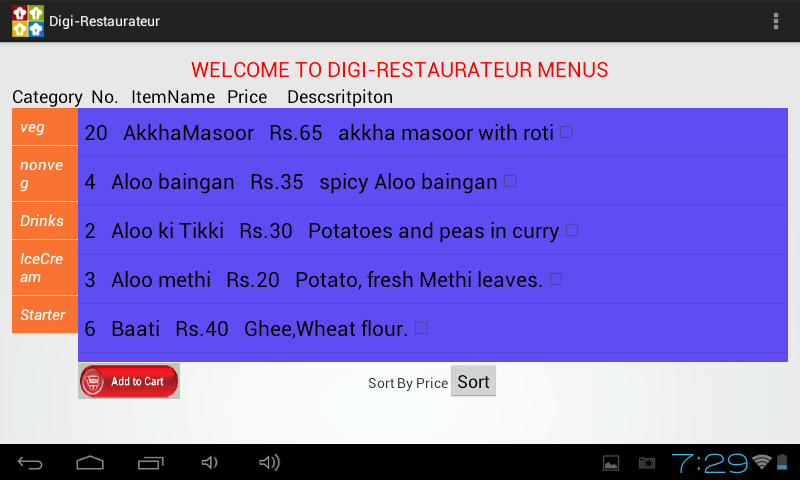
\includegraphics[width=5in]
{t3}
\caption{Menu Selection window}
\end{figure}


\begin{figure}[h!]
\centering
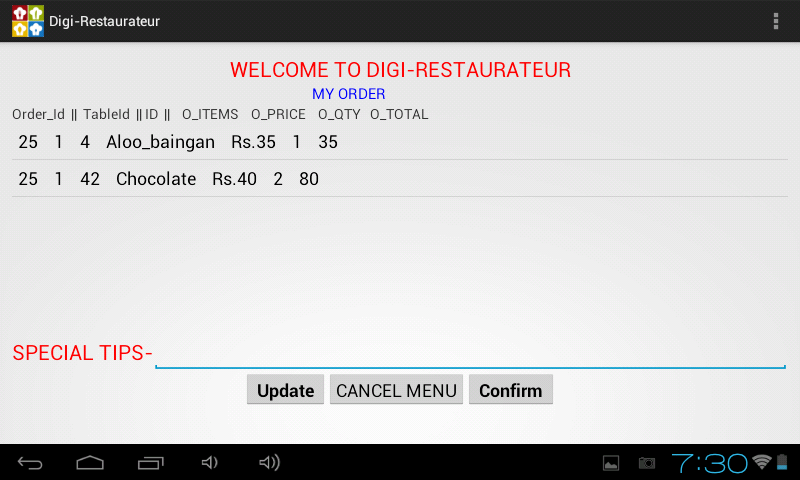
\includegraphics[width=5in]
{t4}
\caption{Confirm and update  panel}
\end{figure}

\begin{figure}[h!]
\centering
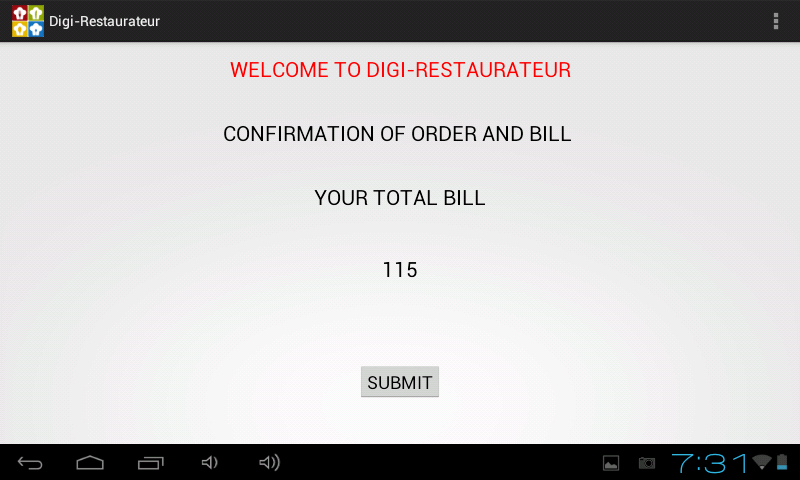
\includegraphics[width=5in]
{t5}
\caption{submit orders window}
\end{figure}



\begin{figure}[h!]
\centering
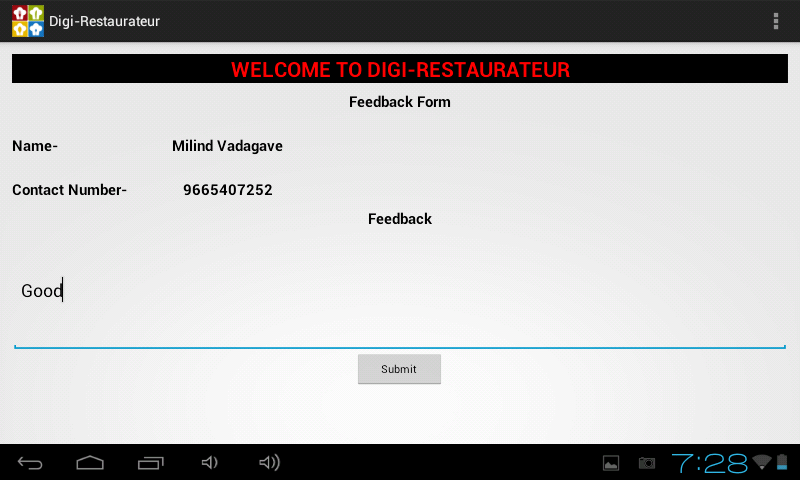
\includegraphics[width=5in]
{t9}
\caption{feedback window}
\end{figure}
















